\documentclass[a4paper,11pt]{article}
\usepackage{exptech}
\usepackage{textcomp}
\usepackage{graphicx}
\usepackage{array}
\usepackage[babel=true]{csquotes}
\usepackage{url}
\usepackage{hyperref}
\usepackage{wrapfig}
\usepackage[export]{adjustbox}
\usepackage{titletoc}

\hypersetup{
  %bookmarks=true, % show bookmarks bar?
  pdftitle={Avalon - Rapport de pré-étude}, % title
  pdfnewwindow=true, % links in new window
  colorlinks=true, % false: boxed links; true: colored links
  linkcolor=black, % color of internal links (change box color with linkbordercolor)
  citecolor=cyan, % color of links to bibliography
  filecolor=cyan, % color of file links
  urlcolor=cyan % color of external links
}

\title{
  \textbf{Avalon}\\
  Rapport final
}
\markright{Avalon - Rapport final}
\author{
\begin{minipage}{0.4\textwidth}
	\begin{flushleft} \large
		\emph{Auteurs :}\\
		Alexandre \textsc{Audinot}\\
		Julien \textsc{Bouvet}\\
		Thierry \textsc{Gaugry}\\
		Nicolas \textsc{Hurman}\\
		Alexandre \textsc{Leonardi}\\
	\end{flushleft}
\end{minipage}
\begin{minipage}{0.4\textwidth}
	\begin{flushright} \large
		\emph{Encadrants :} \\
		Valérie \textsc{Gouranton}\\
		Ronan \textsc{Gaugne}\\
		Bruno \textsc{Arnaldi}\\
		Willy \textsc{Allègre}\\
		Jean-Paul  \textsc{Departe}\\
	\end{flushright}
\end{minipage}
}

\date{26 mai 2015}

\begin{document}
\maketitle
\thispagestyle{empty}
\begin{abstract}
\textbf{Avalon :} Environnement de Réalité Virtuelle pour l'apprentissage à l'utilisation d'appartements tremplins. Réalisation en 3D d'un appartement domotisé interactif utilisé dans le cadre de la rééducation des personnes handicapées.\newline

Le projet est proposé par le centre mutualiste de rééducation et de réadaptation fonctionnelles de Kerpape (plus particulièrement les ingénieurs du laboratoire électronique Willy Allègre et Jean-Paul Departe).\newline

Le modèle 3D de l'appartement nous est fourni, et notre travail consiste à réaliser un logiciel fonctionnel permettant de se déplacer dans l'appartement et implémentant les interactions avec les différents éléments de domotique, en plus de prendre en charge différents périphériques de contrôle. 
\end{abstract}

\begin{figure}[h!]
	\centering
	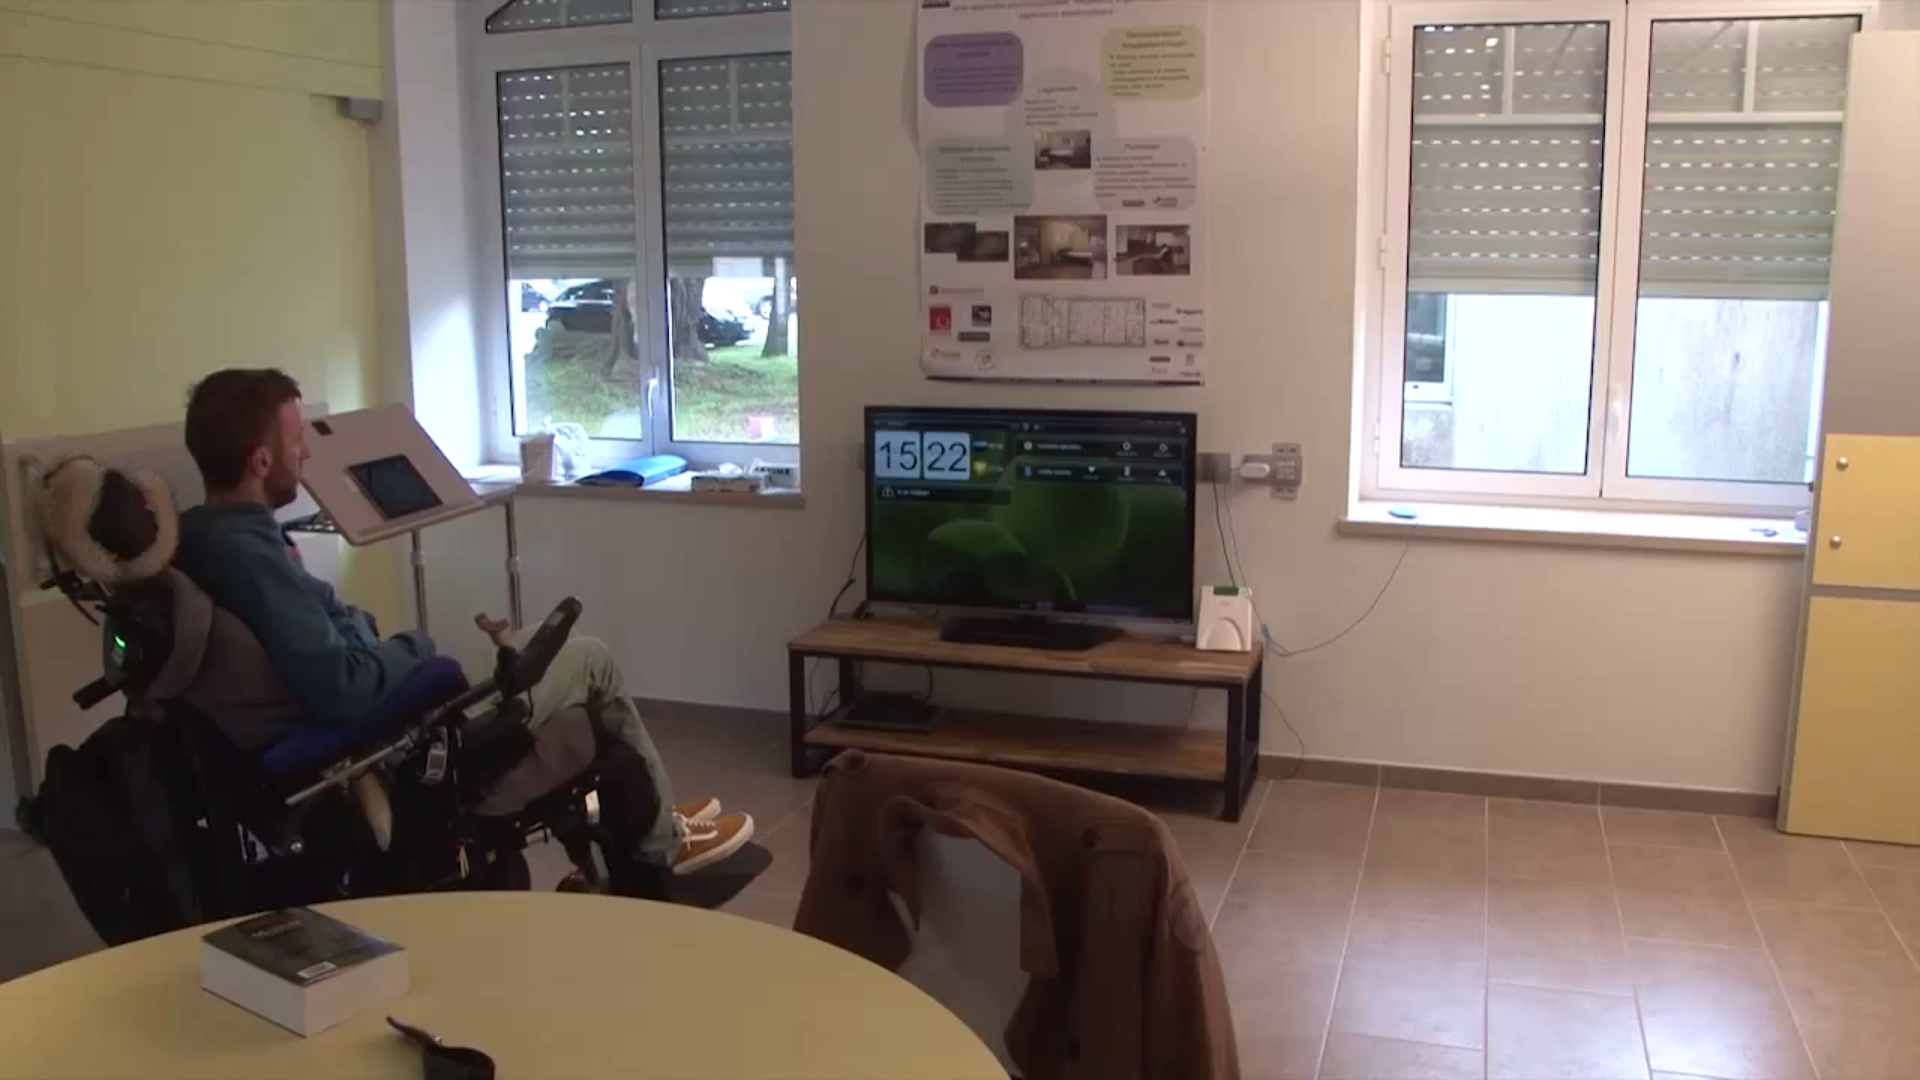
\includegraphics[height=170pt]{7-RapportFinal/img/screen_appart.png}
\end{figure}

%\vfill
%[width=\textwidth]
\begin{figure}[h!]
   \begin{minipage}{0.3\linewidth}
      
\includegraphics[scale=0.9]{7-RapportFinal/img/logo_insa.jpeg}
   \end{minipage} 
   \begin{minipage}{0.2\linewidth}
      \centering
      
\includegraphics[scale=0.5,left]{7-RapportFinal/img/logo_irisa.jpg}
   \end{minipage}\hfill
   \begin{minipage}{0.2\linewidth}
      
\includegraphics[scale=0.9]{7-RapportFinal/img/logo_kerpape.png}
   \end{minipage}
\end{figure}

\pagebreak

\tableofcontents
\pagebreak
\section{ANNEXE I : Tests}

\subsection{Tests unitaires}
L'architecture de notre projet, qui utilise le moteur de jeu Unity3D, ne nous a pas permis d'en faire ! \newline

Les tests unitaires, le type de tests que nous avons le plus utilisés au long de notre formation, fonctionnent très bien avec des projets ne comportant que du code informatique, car ainsi nous aurions pu tester chaque bloc du projet indépendament avant de les assembler entre eux. \newline

Dans le cas de Unity, l'écriture de code n'intervient que dans les scripts en C\# qui ne représentent pas l'intégralité du projet. De plus, leur utilisation étant intimimement mêlée aux actions de l'utilisateur dans l'univers 3D, il était impossible de les tester indépendament. \newline

Unity propose tout de même un ensemble d'outils de test, qui permet entre autres choses de réaliser des tests unitaires, mais les délais du projet ne nous ont pas permis de prendre en main cesoutils. Les tests que nous avons réalisé au long de notre projet sont donc principalement des tests fonctionnels et d'acceptation. 

\subsection{Tests fonctionnels}

Les tests fonctionnels représentent la majorité de ceux que nous avons menés au cours du projet Avalon. Faciles à mettre en place, ils nous assuraient qu'une modification n'entraîne pas une régression nattendue. Nous vérifiions chaque fonctionnalité indépendament, sans prendre la peine de mettre en place une scénario d'utilisation réaliste mais simplement en vérifiant que le programme répondait de la manière souhaitée à une situation donnée (conformité aux spécifications du projet).\newline

Chaque fonctionnalité, au moment de son intégration, a été dûment testée, ainsi qu'à plusieurs reprises par la suite à chaque fois qu'une modification était suceptible de l'impacter. À titre d'exemple, nous avons testé les déplacements au clavier/souris quand nous avons créé le script utilisé, puis plus tard quand nous avons modifié la manière de contrôler la wand qui fait office de curseur à l'écran et requérait une attention particulière, ou encore quand nous avons créé une zone où l'utilisateur perdait le contrôle de ses déplacements et était déplacé « sur des rails ».\newline

L'avantage principal de ce type tests est leur facilité, et ils nous permettent de tester chaque fonctionnalité indépendament et en temps réel, mais en contrepartie nous courrions le risque de ne pas remarquer cetains cas d'erreurs qui ne seraien pas apparus clairement, d'une part parce qu'étant les concepteurs des fonctionnalités en question nous avions un \textit{a priori} quant à la façon dont il fallait s'en servir, et d'autre part car nous n'avions pas le temps de réfléchir à tous les cas exotiques qui pourraient survenir. 

\subsection{Tests d'acceptation}

Les tests d'acceptation représentent la seconde catégorie de tests que nous avons appliqués. Moins fréquents que les tests fonctionnels, ils sont plus intensifs. \newline

Les tests d'acceptation vérifient le fonctionnement en interaction d'un grand nombre de \textit{features} et sanctionnent une avancée significative du projet. Il s'agit généralement de tester un scénario d'utilisation réaliste qu'un usager serait suceptible de réaliser par lui-même sans connaître les détils d'implémentation du projet. \newline

Pour repredre les exemples du point précédent, une fois toutes les fonctionnalités mentionnées disponibles, nous avons essayé d'apparaître dans la scène, se déplacer librement quelques instants, puis se rendre dans la zone où l'on perdait le contrôle du personnage et en repartir, le tout sans qu'il n'y ait de bug de collision (e.g. traverser un mur ou se glisser dans l'interstice d'une porte). 
\pagebreak
\section{Modification des spécifications}
\subsection{Accessibilité du panneau d'interrupteurs}
A la suite d'une visite, nous avons confirmé avec nos clients de Kerpape qu'il était difficile d'accéder aux boutons du panneau de commandes dans l'application. A cause de leur taille, il fallait beaucoup de précision pour appuyer sur un bouton et non son voisin. Nous avons donc implémenté un système pour faciliter la visée de l'utilisateur en affichant les interrupteurs plus proches de la caméra.\newline

Lorsque l'utilisateur s'approche du panneau de commande, la caméra se déplace linéairement pour que les interrupteurs soient au centre de l'écran. De cette manière, les étiquettes sont plus visibles, et il est plus facile d'appuyer sur les boutons.\newline

A ce moment, les déplacements sont bloqués ainsi que la caméra. Lorsque l'utilisateur déplace la souris, le curseur se mouvoit de haut en bas et de gauche à droite. L'utilisateur peut ainsi actionner le bouton qu'il souhaite facilement. Pour sortir de ce mode bloqué, il faut appuyer sur la touche directionnelle bas ou 'S', comme pour s'éloigner du mur.

\begin{figure}[h]
	\centering
		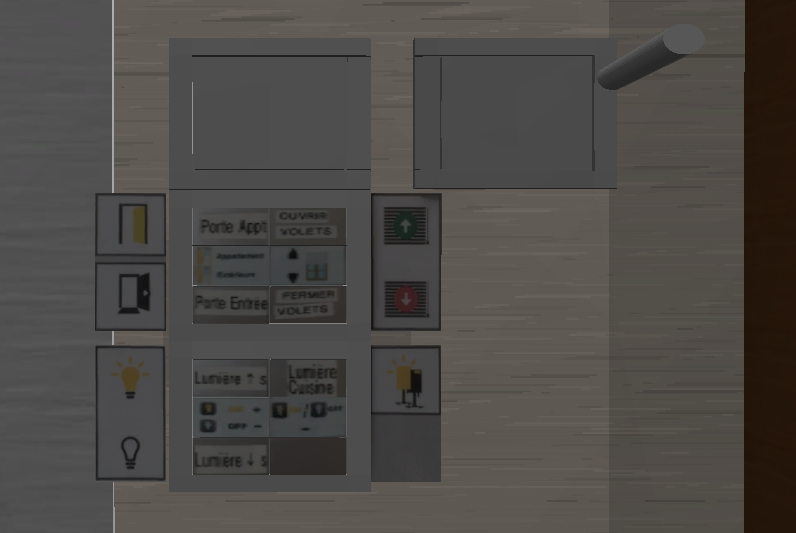
\includegraphics[width=\textwidth]{7-RapportFinal/img/screenshot_panneau_commande.png}
		\caption{Aperçu du panneau de commande dans l'application}
	\label{fig:panneau_commande}
\end{figure}

\pagebreak
\section{Modification dans la conception}

Au cours du projet, nous avons réalisé un schéma de conception logicielle, expliquant comment s'organisaient les scripts les uns par rapport aux autres.
Tout au long de l'implémentation, et bien que nous ayons gardé  en tête le schéma initial, certains facteurs ont fait diverger la conception logicielle réelle de celle prévue.
Parmi ces facteurs, on compte notamment Middle VR et Unity.

\subsection{Middle VR : des imprévus au programme}

Middle VR est une couche logicielle d'abstraction permettant de développer une solution logicielle et de l'utiliser telle quelle avec n'importe quel périphérique de réalité virtuelle.
Il permet, sans modifier la solution, de l'utiliser indifféremment avec un casque de réalité virtuelle ou la faire fonctionner en salle immersive.
Néanmoins Middle VR pose quelques problèmes lorsque l'on veut l'utiliser avec un couple clavier/souris - qui n'est pas un adapté à la réalité virtuelle.
Par exemple, les valeurs de position/rotation de certains objets sont gérés par Middle VR (par exemple le VR Center Node, Head Node, ...). \\
De plus, Middle VR fonctionne en mode tracker : il capte la position des périphériques pour positionner l'utilisateur dans la scène.
Or, si on est physiquement limité (dans une salle immersive par exemple) avec des périphériques de réalité virtuelle, cela n'est pas le cas avec une souris par exemple.
En effet, rien n'empêche l'utilisateur de soulever la souris pour la reculer et donc avancer en continu, et ceci peut poser certains problèmes dans un logiciel de réalité virtuelle.  

\begin{figure}[h]
	\centering
		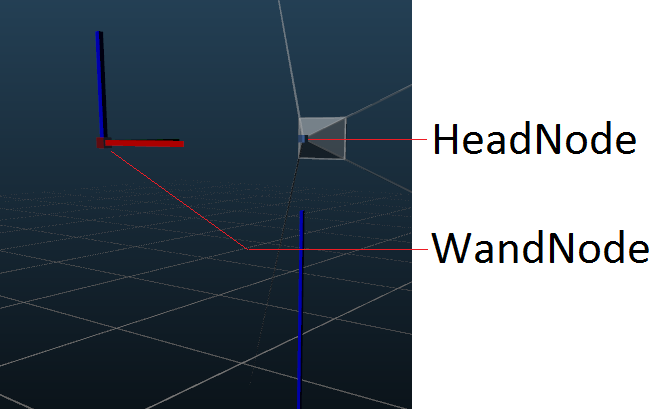
\includegraphics[width=\linewidth]{7-RapportFinal/img/middleVR.PNG}
		\caption{Nodes Middle VR}
		\label{middleVR}
	
\end{figure}

\subsection{Unity : Programmation orientée composants}

Unity fonctionne avec des scripts C\#, attachés en tant que composants sur des objets de la scène (des GameObject).
Pour cela, Unity a son propre compilateur, et son comportement peu parfois être limitant.
Par exemple l'utilisation de pointeurs, bien que fortement déconseillée en C\#, est presque impossible avec Unity. De plus, de par son fonctionnement (orienté composants), l'héritage pose des problèmes sur les scripts qui ont des fonctions update et start.
En effet, start est une fonction lancée - après les constructeurs - au lancement du script, et Update est appelée une fois par frame.
Or, une fonction update ou start peut nécessiter l'éxécution de celle d'un autre script. Pour ces raisons (entre autres), les classes ont du être adaptées.

\subsection{Classes conservées}

Sur le diagramme de classe ci-dessus, la ligne rouge est une démarcation entre les classes qui sont restées presque inchangées dans l'implémentations, et celles qui ne sont pas représentées ou qui ne présentent plus les même caractéristiques. En haut de ladite ligne rouge, sont les classes préservées dans l'implémentation : en effet, la plupart sont abstraites et ne dépendent que des classes standard d'Unity.

\begin{figure}[h]
	\centering
		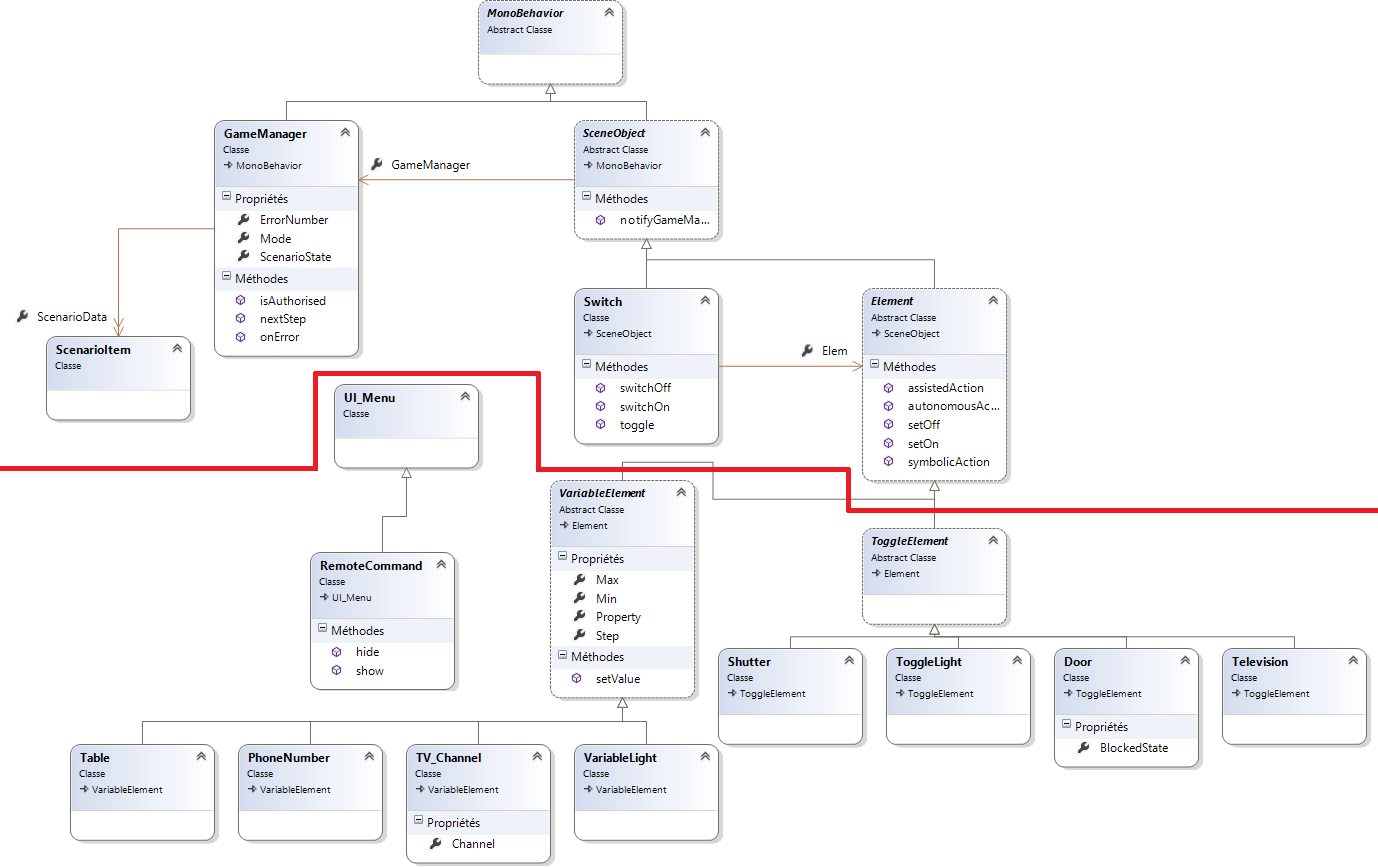
\includegraphics[width=\linewidth]{7-RapportFinal/img/diagClasses_rectif.png}
		\caption{Diagramme de classe initial}
		\label{diagClasses_rectif}
	
\end{figure}

Globalement, même si certaines classes ont disparues ou dont été modifiées, l'architecture générale du projet est respectée. L'ensemble est cohérent avec le schéma initial, même s'il n'est pas rigoureusement identique.







\pagebreak
\section{Realisation du cahier des charges}
Nous avons eu l'occasion d'échanger avec les membres de Kerpape, ce qui nous a permis de définir le cahier des charges de l'application, que nous allons détailler dans cette partie. \\

\subsection{Général}

\begin{tabular}{|p{13cm}|c|}
	\hline
	Tache & Etat \\ \hline
	Afficher l'appartement en 3D & Réalisé \\ \hline
	Deplacement dans l'appartement & Réalisé \\ \hline
	Vue exocentrée : Une vue à la troisième personne permet de voir le déplacement de l'utilisateur dans la scène. & Réalisé \\ \hline
	Vue endocentrée : Une vue à la première personne permet de voir par les yeux de l'avatar  virtuel. & Réalisé \\ \hline
	Interactions : L'utilisateur doit pouvoir interagir avec son environnement (portes, lumières, volets). & Réalisé \\ \hline
	Relancer la scène & Réalisé \\ \hline
\end{tabular}
	
\subsection{Implémenter différents mode de jeu}
\begin{tabular}{|p{13cm}|c|}
	\hline
	Tache & Etat \\ \hline
	Possibilité de basculer entre les modes en cours de jeu & PIKACHU \\ \hline
	Mode symbolique : mise en évidence d'actions à réaliser, ainsi que des indications visuelles symboliques. & Réalisé \\ \hline
	Mode assisté : lors de l'activation d'une action on accède à une vue fixe avec les états courants des équipements afin de faciliter la compréhension du lien action/objet pour l'utilisateur & Réalisé \\ \hline
	Mode autonome : L'utilisateur ne reçoit plus d'information ou d'indication pour effectuer son parcours, il est dans le décor le plus réaliste possible, pour valider son autonomie. Il doit alors actionner les différents objets et se rendre compte par lui même (déplacement) des actions qu'il a effectuées.  & Réalisé \\ \hline
\end{tabular}
		

\subsection{Implémenter différents scenarios de jeu}		
\begin{tabular}{|p{13cm}|c|}
	\hline
	Tache & Etat \\ \hline
	Scenario 1 - Appel téléphonique : Appel téléphonique (d'un proche ou d'une personne qui se serait trompée de numéro). L'utilisateur doit pouvoir décrocher le téléphone pour entrer en communication puis raccrocher quand la communication est terminée. & Réalisé \\ \hline
	Scenario 2 - Interphone infirmier : Appel venant du portier audio/vidéo sur le téléphone (d'un infirmier qui souhaiterait entrer). L'utilisateur doit pouvoir décrocher le téléphone, communiquer avec l'infirmier, raccrocher le téléphone et ouvrir la porte.& Réalisé \\ \hline
	Scenario 3 - Interphone inconnu : Appel venant du portier audio/vidéo sur le téléphone (d'un inconnu). L'utilisateur doit pouvoir décrocher le téléphone pour entreren communication, allumer la TV pour voir la vidéo puis éteindre la TV et raccrocher le téléphone à la fin de la conversation.& Réalisé \\ \hline
\end{tabular}
		

\subsection{Portabilité}
\begin{tabular}{|p{13cm}|c|}
	\hline
	Tache & Etat \\ \hline
	Application portable - faire une application aisément portable sur différents systèmes d'utilisation & Windows seulement \\ \hline
	Capable de fonctionner avec de nombreux périphériques différents & Utilise MiddleVR \\ \hline
	Salle immersive & Fonctionnel dans Immersia \\ \hline
	Porter le logiciel sur tablette  & NOPE.JPG \\ \hline
	Casque de réalité virtuelle & Réalisé \\ \hline
	Clavier souris & Réalisé \\ \hline
\end{tabular}

\pagebreak
\input{7-RapportFinal/manuelUtils.tex}



\end{document}
